\section{Simulated Annealing a rozkład kanoniczny}
%%%%%%%%%%%%%%%%
	
	\begin{frame}{Simulated Annealing a rozkład kanoniczny}
		\textbf{Własności makroskopowe z mikroskopowymi}
		\begin{itemize}
			\item Q - stan mikroskopowy układu
			\item E(Q) - energia układu w stanie Q
			\item P(Q) - rozkład prawdopodobieństwa 
			\item Rozkład mikrokanoniczny - układ izolowany
		\end{itemize}
		$$
		P(Q) = A(Q) \cdot \delta(E - E(Q))
		$$
		$$
		A(Q) = \begin{cases}
		0 - \text{niemożliwe} \\
		1 - \text{możliwe}
		\end{cases}
		$$
	\end{frame}

\subsection{Rozkład kanoniczny}

%%%%%%%%%%%%%%%%
	\begin{frame}{Simulated Annealing a rozkład kanoniczny}
		\begin{block}{Rozkład kanoniczny}
			Układ w kontakcie cieplnym z otoczeniem
		\end{block}
		
		\begin{figure}
			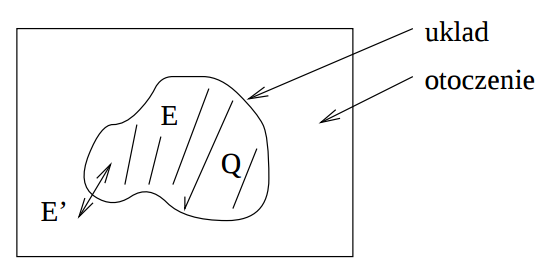
\includegraphics[width=0.35\textwidth]{img/18/canonical_distribution}
		\end{figure}
		
		$$
		P(Q) = Z^{-1} \cdot e^{-\frac{E(Q)}{kT}}
		$$
		
		$$
		\sum_Q P(Q) = Z^{-1} \cdot \sum_Q e^{-\frac{E(Q)}{kT}} = 1 \Rightarrow \underbrace{Z = \sum_Q e^{-\frac{E(Q)}{kT}}}_{\text{suma statystyczna - fukcja rozdziału}}
		$$
		
		często: $\frac{1}{kT} = \beta$
	\end{frame}

%%%%%%%%%%%%%%%%
	\begin{frame}{Ciepło właściwe}
		E = Var
		\begin{block}{$ <E> = U \rightarrow$ energia wewnętrzna: można ją zmierzyć}
			$$
			< E >\sum_Q E(Q) \cdot P(Q) = \dfrac{\sum_Q E(Q) \cdot e^{-\beta\cdot E(Q)}}{\sum_Q e^{-\beta\cdot E(Q)}} = - \frac{\partial}{\partial \beta} ln Z
			$$
		\end{block}
	
		\begin{block}{Krócej:}
			$$
			<E> = \frac{\partial}{\partial \beta} ln Z
			$$
		\end{block}	
	\end{frame}
	
%%%%%%%%%%%%%%%%
	\begin{frame}{Ciepło właściwe}
		\begin{block}{Ciepło właściwe przy stałej objętości}
			$$
			C_v = \frac{d<E(T)>}{dT}
			$$
			ale:
			$$
			C_v = \frac{k}{\beta^2}[\underbrace{<E^2(T)>}_{\text{średni kwadrat energii}} - \underbrace{<E(T)>^2}_{\text{kwadrat średniej energii}}]
			$$
		\end{block}		
	
	Wzrost wartości ciepła właściwego sygnalizuje zachodzenie przemiany fazowej.	
	\end{frame}

%%%%%%%%%%%%%%%%
	\begin{frame}{Entropia}
		Oznaczana symbolem \textbf{S}
		$$
		T \cdot dS = dQ \text{ - ciepło dostarczane układowi}
		$$
		
		$$
		V = const
		$$
		
		$$
		T \cdot dS = dU = C_v \cdot dt \rightarrow \frac{ds}{dT} = \frac{C_v(T)}{T}
		$$
		
		\begin{block}{Wzór końcowy na entropię}
			$$
			S(T) = S(T_1) - \int_T^{T_1} \frac{C_v(T')}{T'}dT'
			$$
		\end{block}
		
		\begin{itemize}
			\item $T_1$ - temperatura, dla której entropia jest znana (np. przez aproksymację dla b. wysokich temperatur)
			\item Poziom $S$ $\rightarrow$ ilość minimów (stanów ustalonych)		
		\end{itemize}
	\end{frame}